\chapter{Przegląd istniejących rozwiązań}
\label{ch:przeglad_istniejacych_rozwiazan}

Projektowanie topografii jest obecnie istotnym elementem procesu tworzenia współczesnej elektroniki,
wymagającym zarówno solidnej wiedzy teoretycznej,
jak~i~umiejętności praktycznych korzystania z~odpowiednich narzędzi.
Dostępne na rynku programy wspierające ten proces oferują wiele zaawansowanych funkcji,
ale ich złożoność oraz częsta potrzeba posiadania płatnej licencji ogranicza ich przystępność dla osób początkujących.\\
\indent Istniejące rozwiązania mogą wskazać jakie funkcje, zarówno podstawowe, jak~i~zaawansowane,
powinny zostać zaimplementowane w~programie.
Analiza ich zalet, ograniczeń, jak również przystępności dla użytkowników pozwala określić,
w~jaki sposób unikać problemów z~intuicyjnością i~ergonomią interfejsu jednocześnie wykorzystując sprawdzone mechanizmy.\\
\indent Poza programami do tworzenia schematów należy również przyjrzeć się innym profesjonalnym lub półprofesjonalnym narzędziom,
co pozwoli na zrozumienie,
jak powinien być zaprojektowany schludny i~intuicyjny interfejs użytkownika.

\section{Magic VLSI}

Jednym z bardziej popularnych oraz najbardziej dostępnych programów do projektowania układów scalonych
jest Magic VLSI\@.
Opracowany w 1983 roku przez Johna K. Ousterhouta i jego zespół na Uniwersytecie Kalifornijskim w Berkeley,
napisany w języku C, pierwotnie dla systemu Berkeley 4.2 będącego wariacją platformy Unix~\cite{MAGIC_article}.
Program ten posiada własną stronę internetową, na której można znaleźć dokumentację, kod źródłowy,
wskazówki dotyczące projektowania schematów, jak również pobrać program~\cite{MAGIC_site}.
Dzięki otwartemu kodowi źródłowemu oraz wysokiej funkcjonalności Magic zyskał dużą popularność
w środowiskach akademickich i naukowych, a także wśród hobbystów.
Jego główną jest brak konieczności posiadania płatnej licencji,
przy czym jednocześnie pozwala na pełne zaprojektowanie schematu układu scalonego.\\
\newpage
\indent Unikalną cechą programu Magic jest wprowadzenie techniki strukturyzacji danych
zszytych narożników \textit{corner-stitched},
która znacząco poprawia jego wydajność.
Mechanizm ten opiera się na reprezentacji układu scalonego jako zestaw warstw,
na które składa się zestaw prostokątnych komórek.
%(ang. \textit{cells}).
Każda komórka zawiera zszyte narożnikami powierzchnie (ang. \textit{corner-stitched planes}),
opisujące jej geometrię oraz podkomórki, a każda z nich składa się z wielu prostokątnych kafelków.
Taka struktura pozwala na szybkie i efektywne operacje na schemacie,
takie jak znajdywanie wszystkich kafelek w danym obszarze lub sąsiadów danej komórki,
a także przeszukiwanie połączonych regionów kafelków.
Dzięki zastosowanym mechanizmom możliwe jest także wykonywanie operacji na dużych obszarach
i szybką aktualizację danych.

\begin{figure}[h]
    \centering
    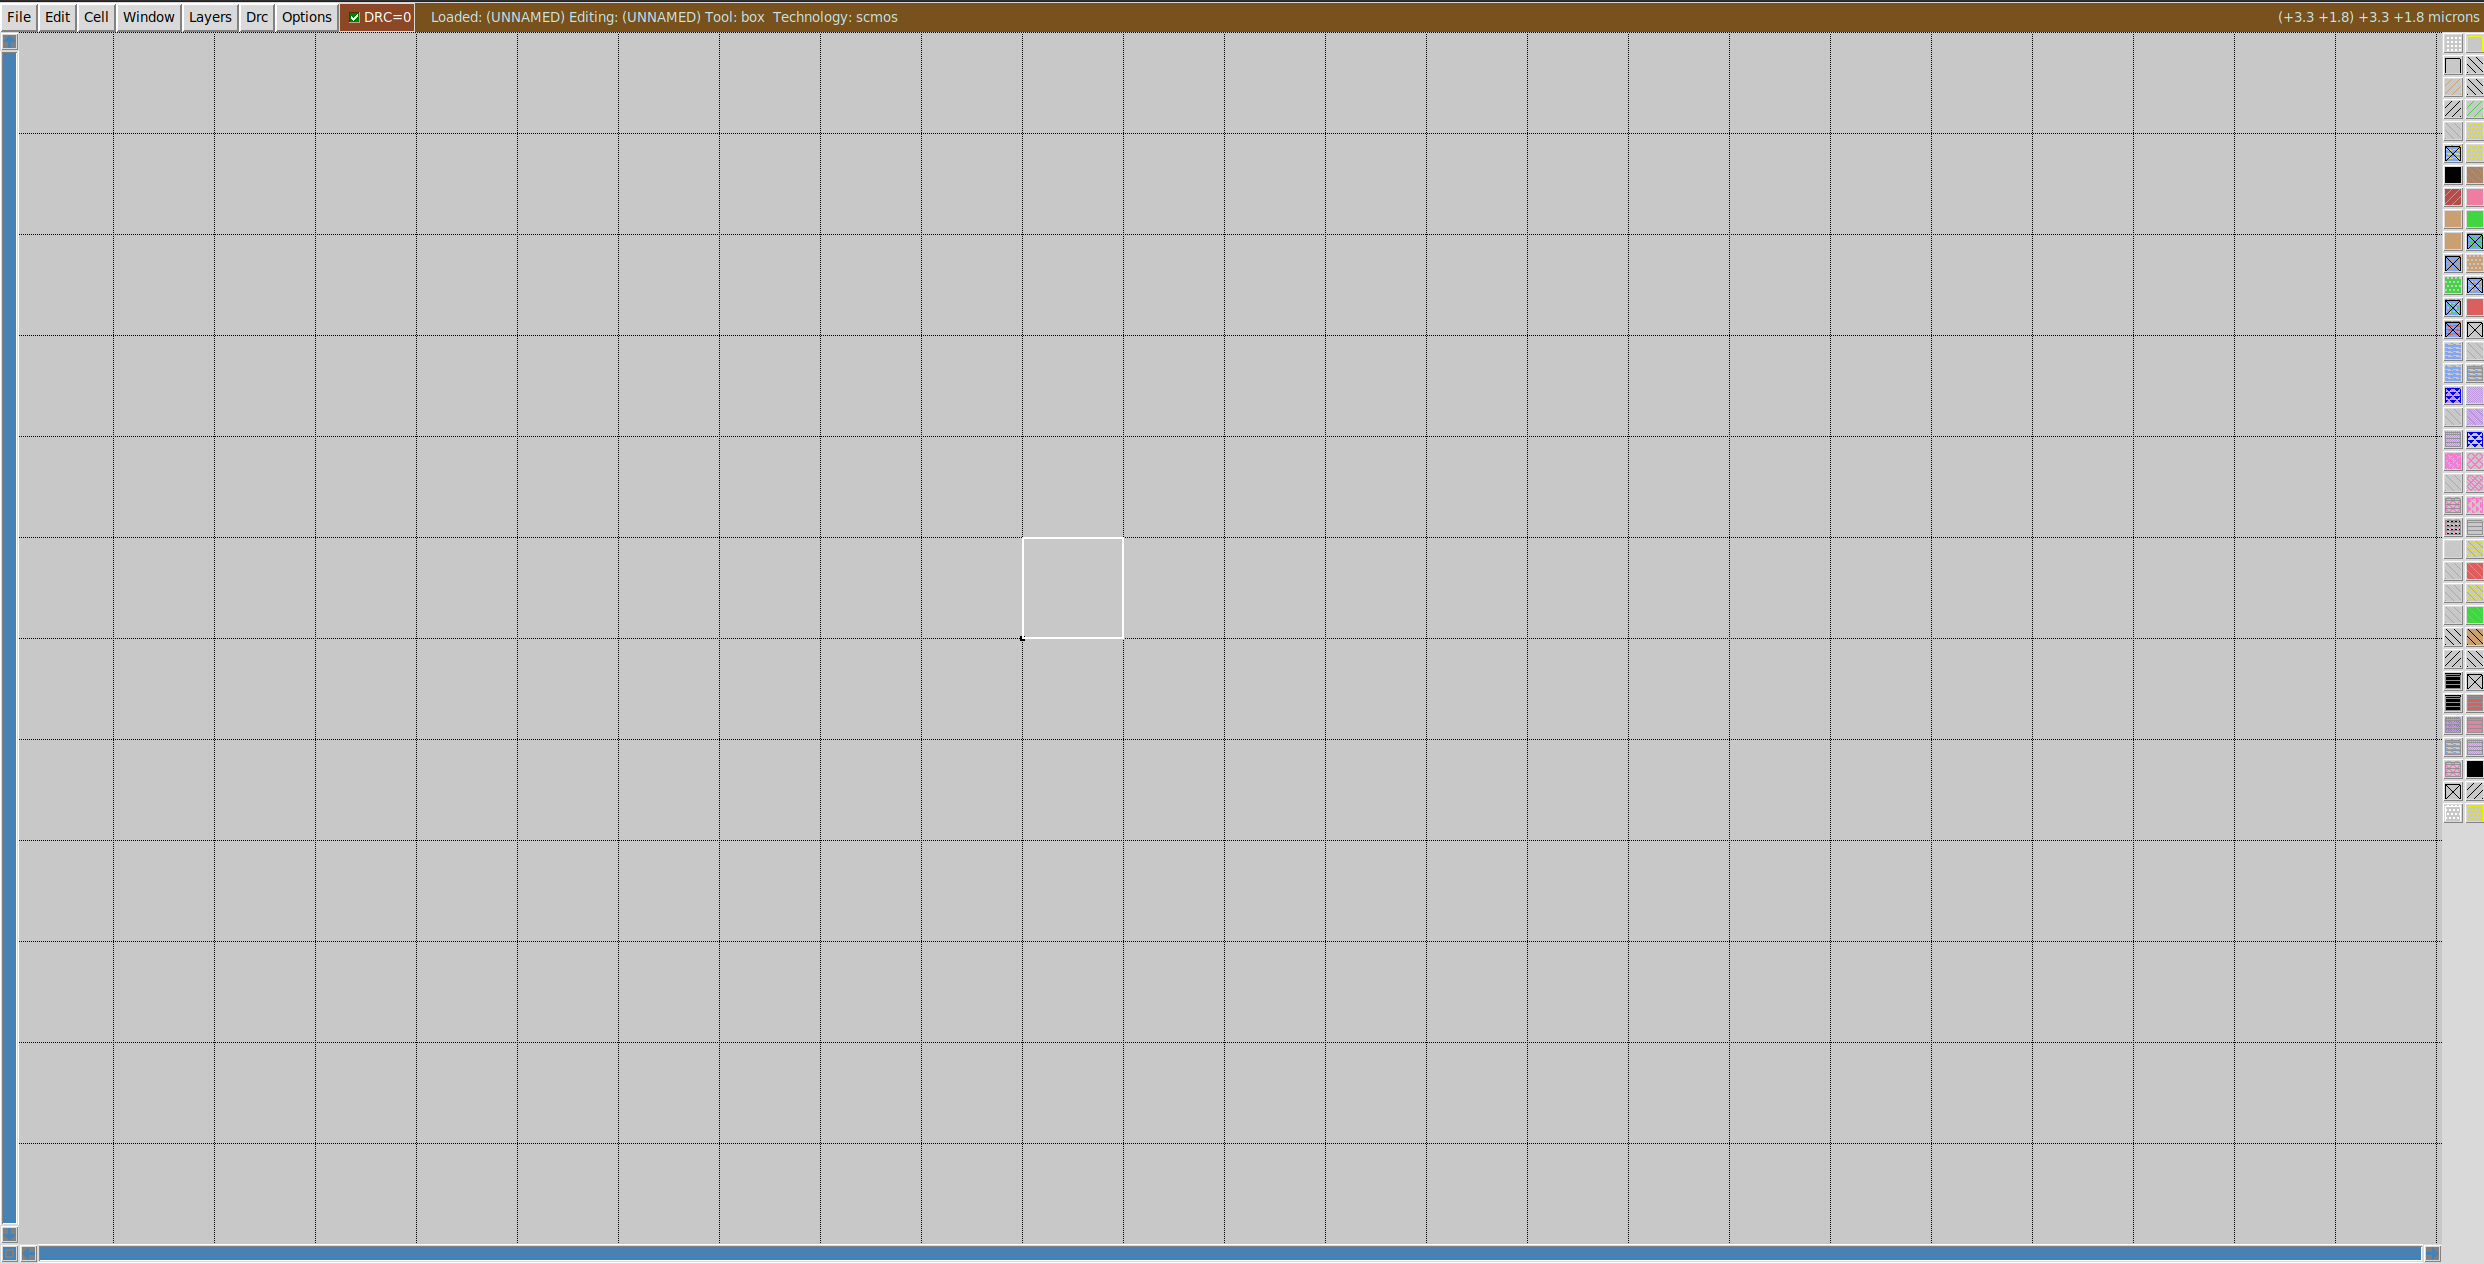
\includegraphics[width=\textwidth]{chapters/chapter2/img/magic_okno}
    \caption{Widok okna programu Magic VLSI.}
    \label{fig:magic_okno}
\end{figure}

\indent Magic VLSI posiada prosty interfejs graficzny,
który składa się z obszaru roboczego, paska narzędzi oraz paska wyboru materiałów.
Dodatkowo wraz z głównym oknem programu otwiera się okno konsoli pozwalające na wprowadzanie dodatkowych komend.
Rysowanie zaczyna się od zaznaczenia obszaru, lewy przycisk myszy służy do wyboru pozycji obszaru,
a prawy do jego rozszerzania.
Aby wypełnić obszar, należy wybrać odpowiedni materiał z paska wyboru
lub z już narysowanych komórek,
poprzez kliknięcie środkowym przyciskiem myszy.
%z tego powodu obecnie można go włączyć jedynie na systemach operacyjnych z rodziny Unix.


\section{Microwind}

Microwind to zintegrowane oprogramowanie należące do rodziny EDA (ang. \textit{Electronic Design Automation}),
służące do automatyzacji procesu projektowania układów scalonych lub płytek drukowanych,
umożliwiające projektowanie, symulacje, weryfikacje oraz testowanie układów elektronicznych~\cite{eda}.
Program ten został opracowany przez dra Sicarda do celów edukacyjnych, składa się z kilku modułów,
odpowiadających za różne etapy projektowania układów scalonych~\cite{Microwind}.
Instalacja w przypadku Microwinda jest prosta, wymaga jedynie pobrania pliku instalacyjnego z oficjalnej strony,
a następnie zainstalowania go na komputerze z systemem Windows~\cite{Microwind},
są to natomiast wersje lite (wersja z ograniczoną funkcjonalnością), pełna wersja wymaga licencji.
Dostępna jest także archiwalna pełna wersja programu, która jest dostępna za darmo~\cite{old_microwind}.
Strona zawiera również dokumentację oraz przykłady projektów,
które można wykorzystać w celach edukacyjnych~\cite{Microwind}.\\
\indent Jednym z modułów programu Microwind jest edytor schematów \textbf{Nano Lambda},
pojawiający się domyślnie po uruchomieniu programu.
Posiada dość nieskomplikowany interfejs graficzny z paskiem menu i narzędzi
oraz pływającym oknem palety warstw, przedstawiony na rys.~\ref{fig:microwind_okno}.

\begin{figure}[h]
    \centering
    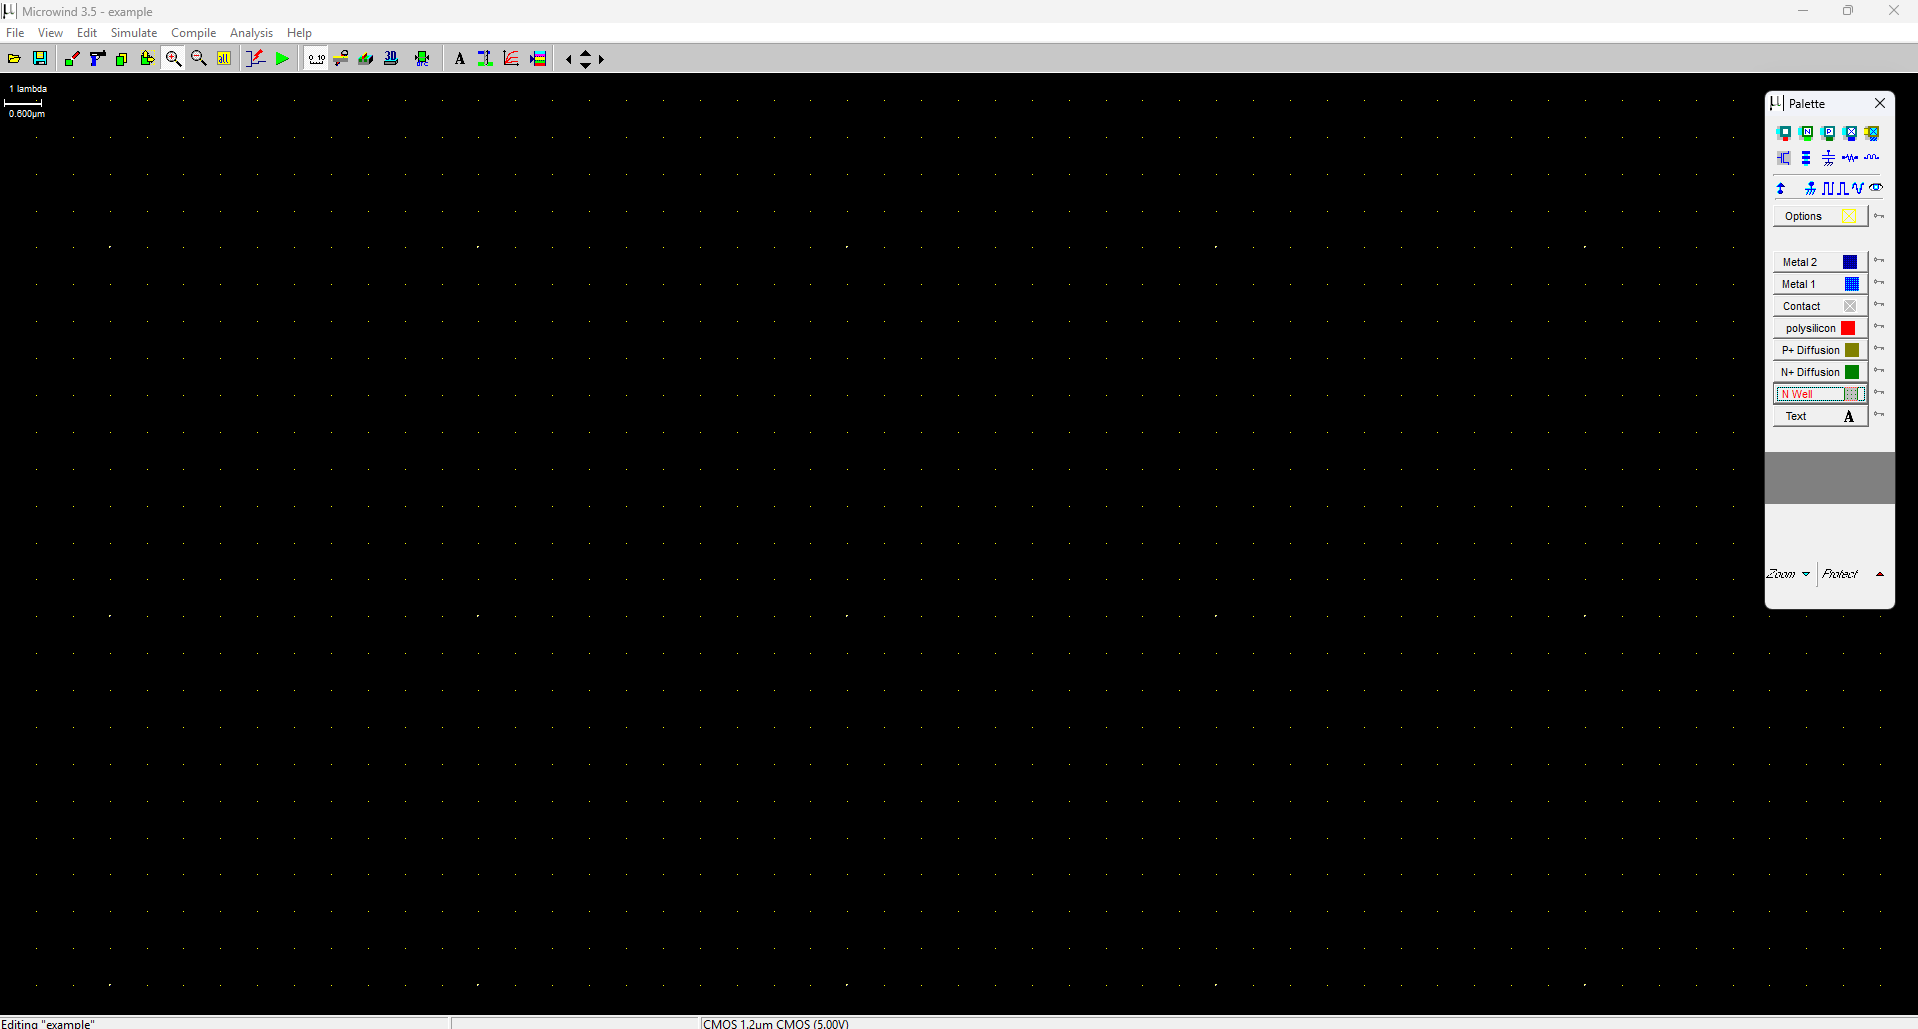
\includegraphics[width=.9\textwidth]{chapters/chapter2/img/microwind_okno}
    \caption[Widok głównego okna programu Microwind.]{Widok głównego okna programu Microwind, źródło:~\cite{Microwind}.}
    \label{fig:microwind_okno}
\end{figure}

\indent Rysowanie odbywa się podobnie jak w przypadku klasycznych edytorów graficznych,
poprzez wybór warstwy z palety,
a następnie przeciągając kursorem po obszarze roboczym przy wciśniętym lewym lub środkowym przycisku myszy,
rysując przy tym prostokątną komórkę.
Nieznaczną wadą rysowania w Microwindzie jest brak przyciągania do siatki,
przez co jest mało precyzyjne.
Przemieszczanie się na obszarze roboczym wymaga używania klawiszy kierunkowych lub przycisków na pasku narzędzi,
co obecnie jest już rozwiązaniem nieergonomicznym.
Program Microwind, poza typowymi narzędziami edycji, charakteryzuje się wieloma zautomatyzowanymi narzędziami,
pozwalającymi generowanie elementów schematów,
na przykład na podstawie funkcji logicznych lub kodu Verilog~\cite{microwind_operation_commands}.\\
\indent Ze względu na brak otwartego kodu źródłowego trudno określić dokładnie zastosowane mechanizmy edytora,
natomiast na podstawie obserwacji można stwierdzić,
że każda edycja schematu wywołuje ponowne rysowanie całego obszaru roboczego,
co jest szczególnie zauważalne podczas usuwania komórek.
Ta sama operacja również wskazuje na strukturę danych, która zakotwiczeniu komórek w kolumnach,
ponieważ po usunięciu obszaru wewnątrz większej komórki, cała kolumna zostaje usunięta.\\
% TODO: poniższe poprawić
\indent Szata graficzna samego edytora charakteryzuje się wysokim kontrastem,
gdzie warstwy są jednolitymi kolorami, częściowo przezroczystymi,
co jest zauważalne, gdy warstwy te się nakładają, przykład przedstawiono na rys.~\ref{fig:microwind_tran}.

\begin{figure}[h]
    \centering
    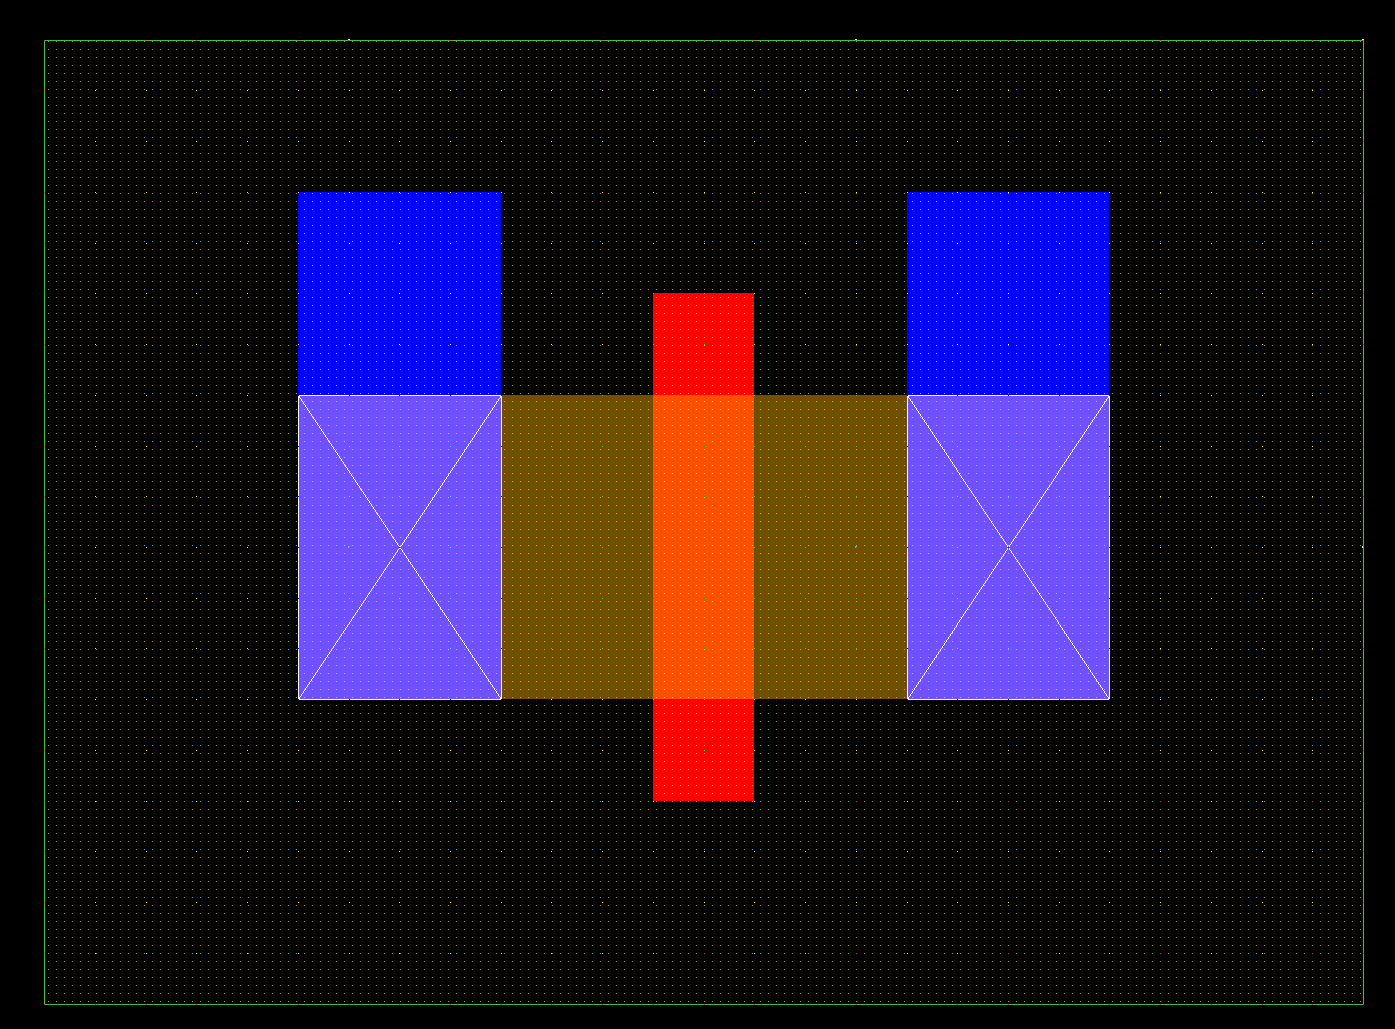
\includegraphics[width=.9\textwidth]{chapters/chapter2/img/microwind_tran}
    \caption[Przykład tranzystora narysowanego w programie Microwind.]
    {
        Przykład tranzystora narysowanego w programie Microwind,
        warstwy \textit{Metal 1}, \textit{P+ Diffusion} oraz \textit{Polysilicon} są jednoilitymi kolorami,
        z wyjątkiem warstwy \textit{N Well} którą reprezentuje kropkowany wzór,
        , źródło: opracowanie własne.
    }
    \label{fig:microwind_tran}
\end{figure}

\section{Electric}
\section{Inne programy}
\label{sec:inne_programy}

Podczas opracowywania oprogramowania,
które spełniać będzie obecne standardy ergonomii i intuicyjności,
warto zwrócić uwagę na inne popularne programy z odrębnych kategorii.
W szczególności będącym na darmowej licencji,
przez co są dostępne dla większej liczby użytkowników
i idealne do nauki danej dziedziny, której dotyczą.

\subsection{GIMP}

Podobnie jak Electric, GIMP jest oficjalnym pakietem GNU i również posiada otwarty kod źródłowy
oraz stosuje założenia wolnego oprogramowania~\cite{gimp_site}.
Jest to program do edycji grafiki rastrowej, \todo

\subsection{Blender}

